%%pruebas con 5 nodos
\chapter{Anexo A}
%%pruebas con 5 nodos

\begin{figure}[!ht]
\centering
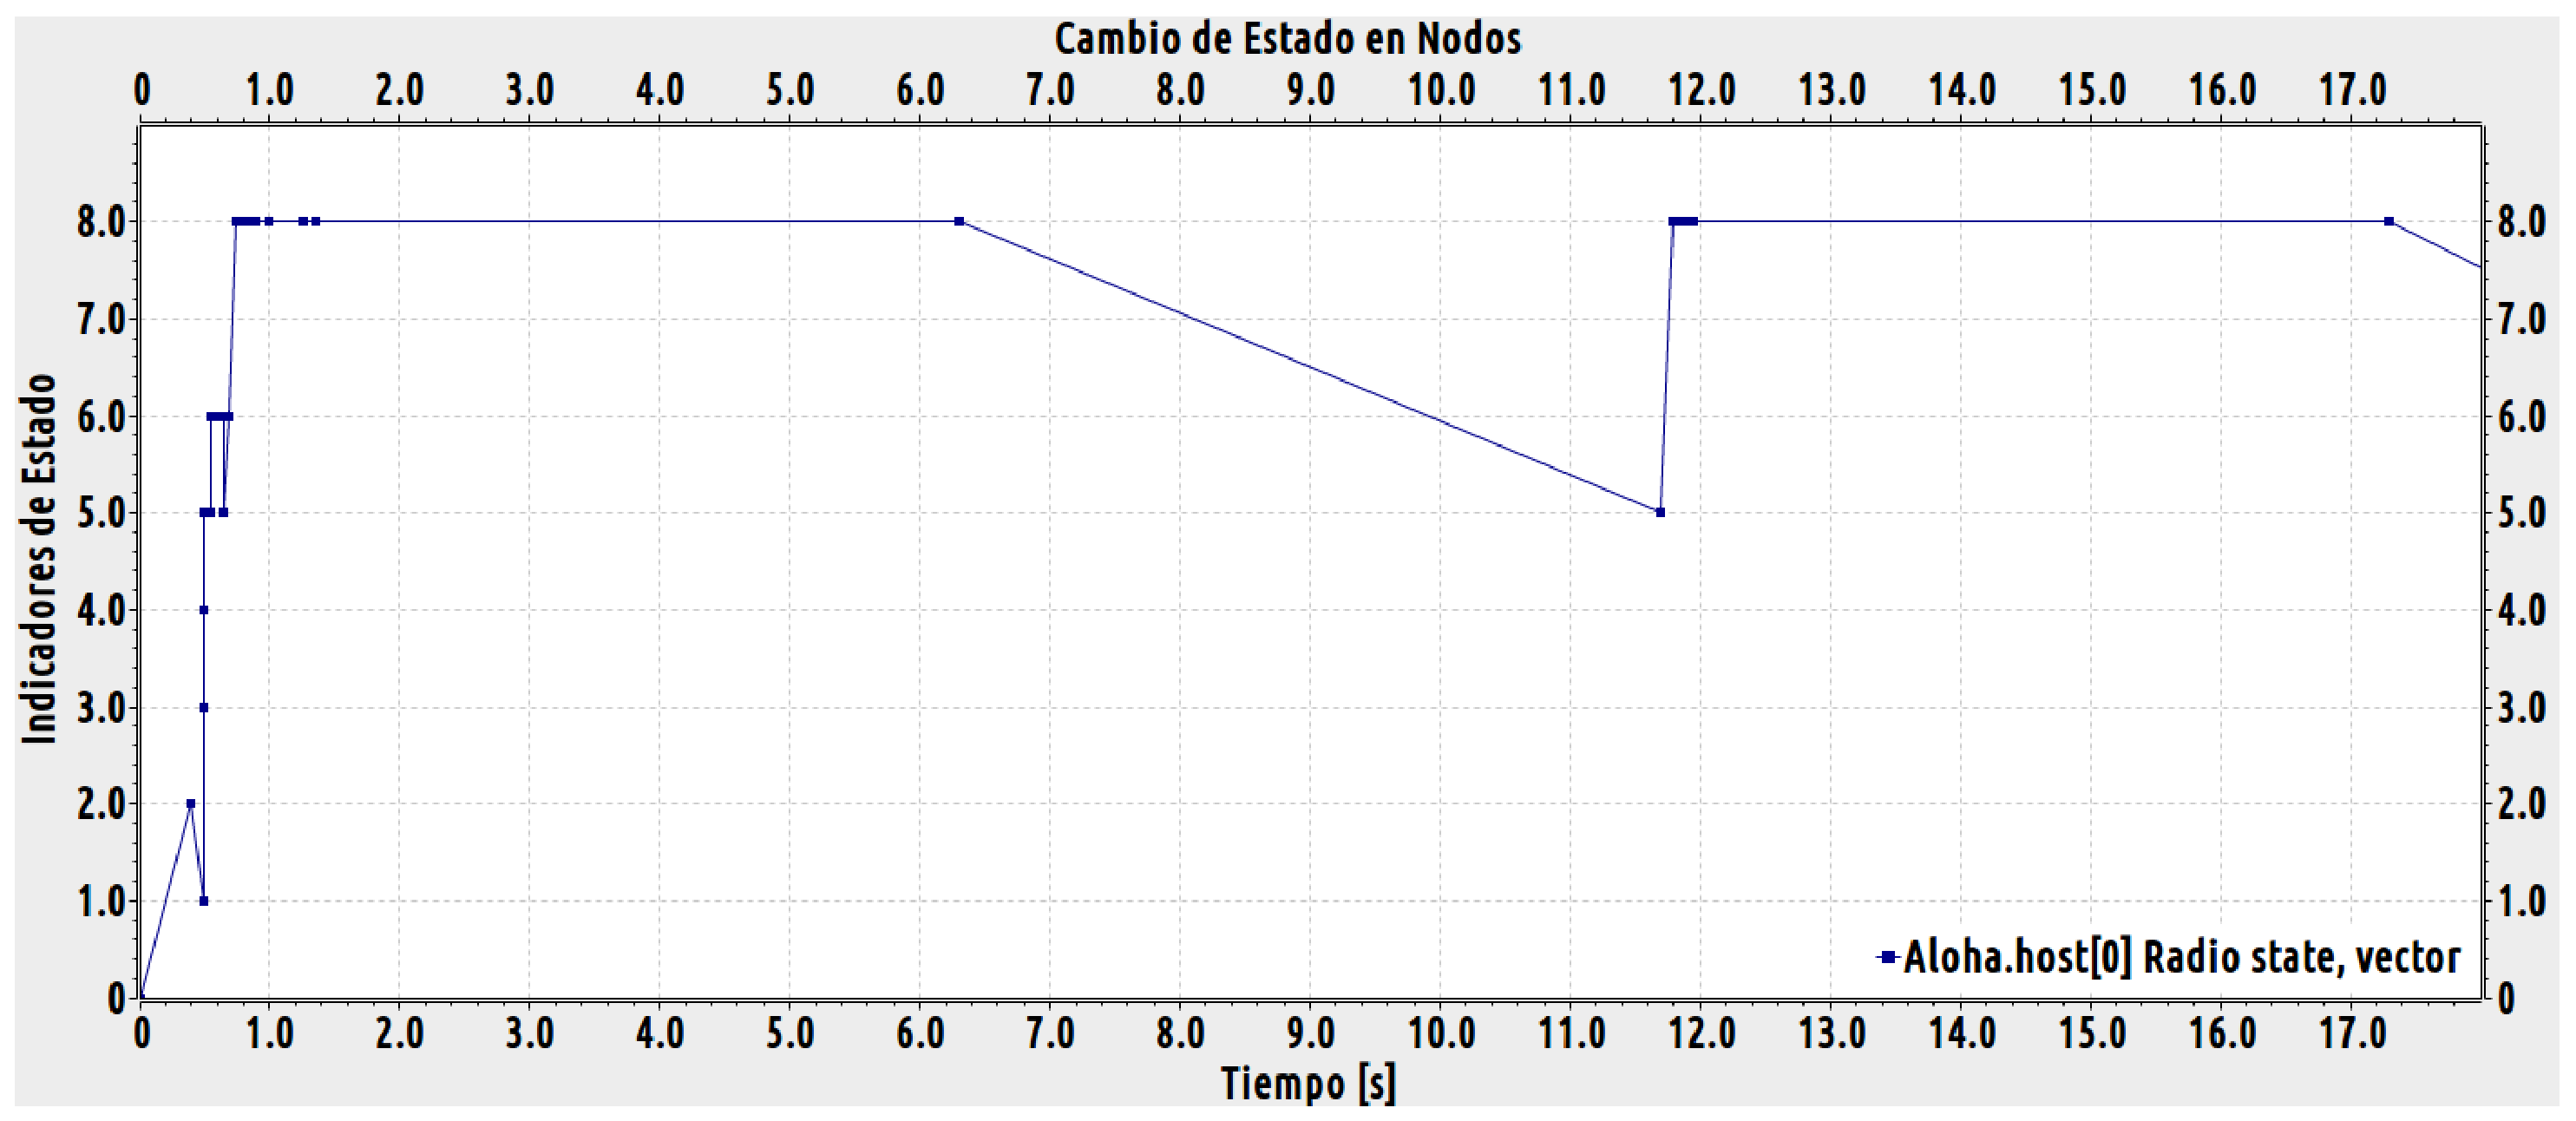
\includegraphics[angle=270, scale=0.4]{images/cambioestado1nodo-ideal.eps}
\caption{Cambios de estados por tiempo en segundos , con un nodos transmitiendo}
\label{anexa:1}
\end{figure}

%% pruebas con 50 nodos
\begin{figure}[!ht]
\centering
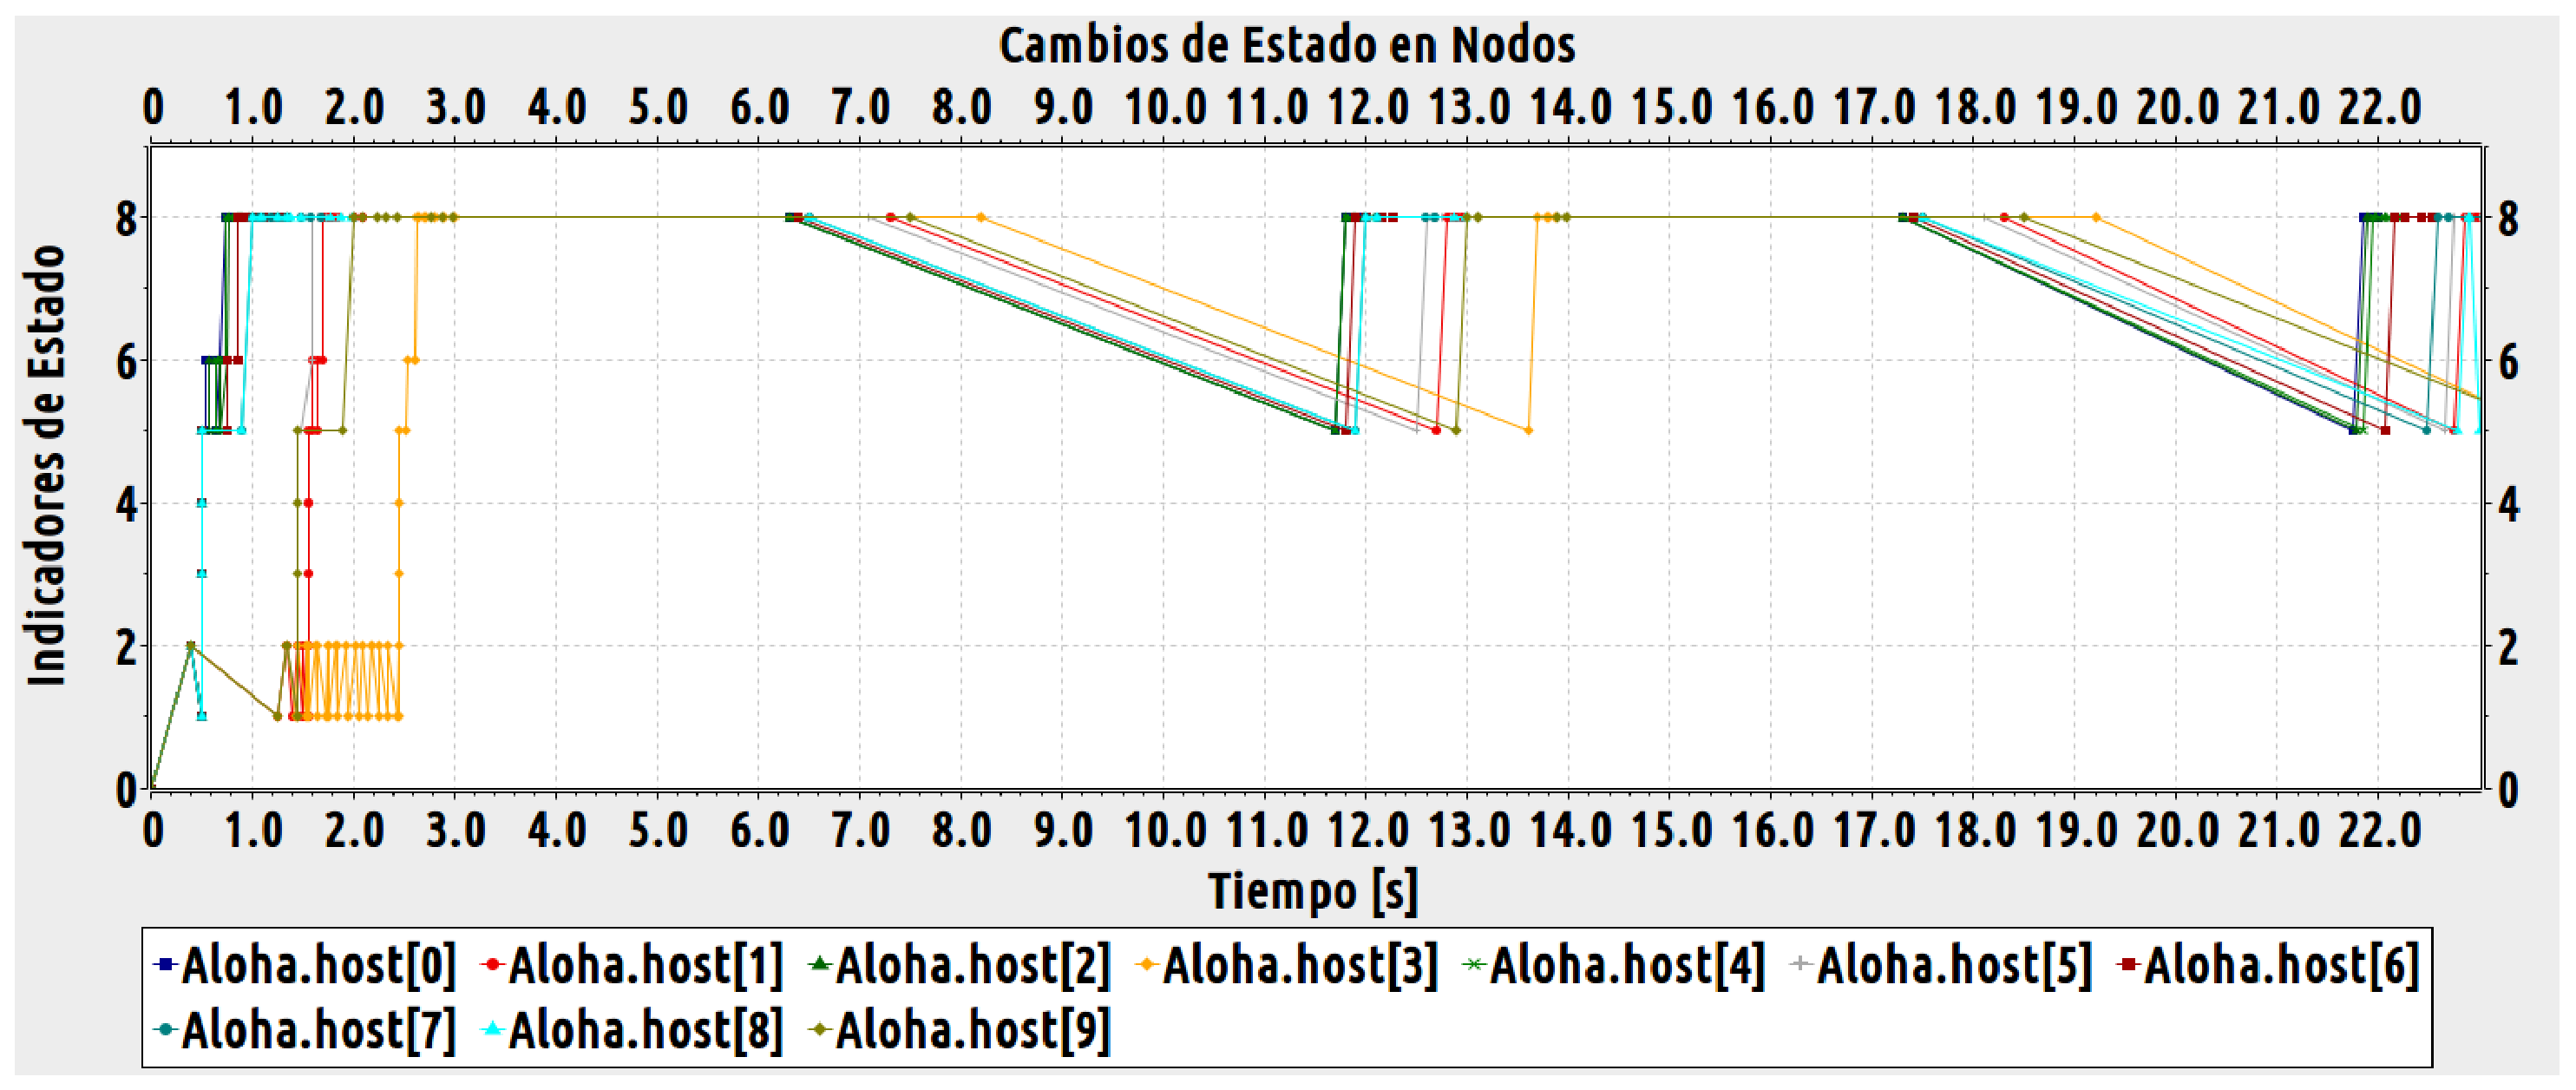
\includegraphics[angle=270, scale=0.4]{images/cambioestado10nodos.eps}
\caption{Gráfico de Cambios de estados por tiempo en segundos , con diez nodos transmitiendo}
\label{anexa:2}
\end{figure}

\begin{figure}[!ht]
\centering
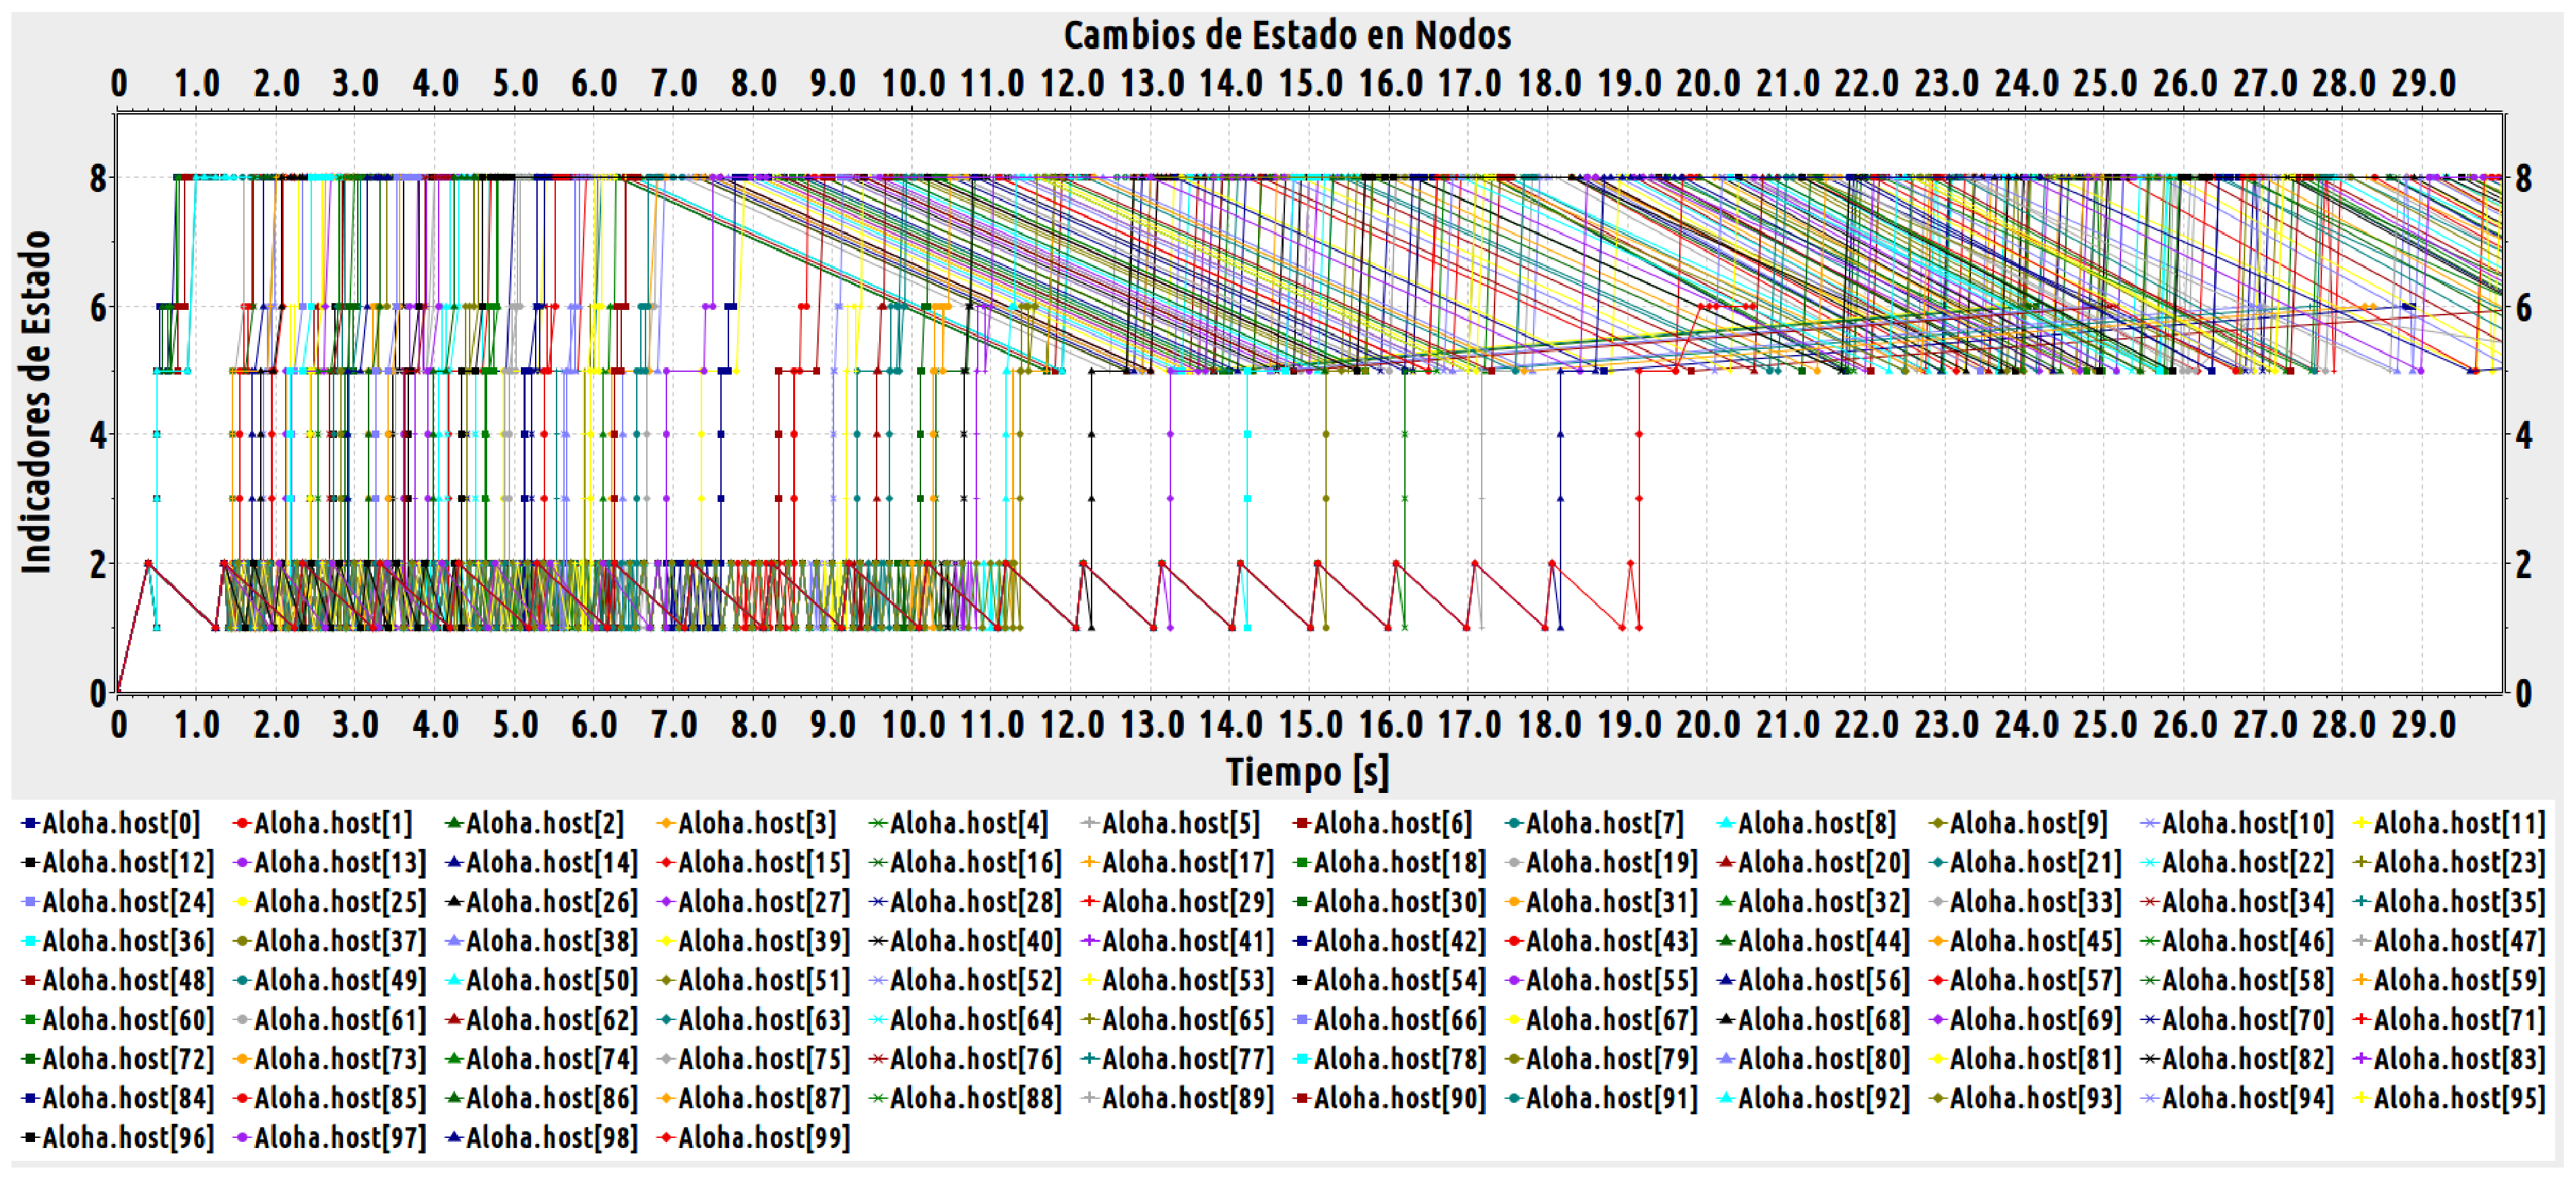
\includegraphics[angle=270, scale=0.4]{images/cambioestado100nodos.eps}
\caption{Gráfico de Cambios de estados por tiempo en segundos , con cien nodos transmitiendo}
\label{anexa:3}
\end{figure}

